
\chapter{Scope}
Die Moduldokumentation beschreibt die Architektur, die Schnittstellen
und die Hauptmerkmale des Moduls. Außerdem werden die Modul bzw. Komponententests
einschließlich der Ergebnisse beschrieben und dokumentiert.
Die MOD dient bei Bedarf auch als Programmier- oder Integrationshandbuch für das
Modul. Wenn bestimmte Risiken direkt mit der Verwendung des Moduls verknüpft sind,
so sind sie in diesem Dokument zu benennen und zu kommentieren.

\chapter{Definitionen}

\section{Abkürzungen}
ESK - Empfänger-Sender-Komponente\\
MTT - Multicast-Test-Tool\\
JCF - Java Concurrency Framework

\section{Definitionen}
Thread - leichtgewichtiger Systemprozess

\chapter{Analyse}
%Dieses Kapitel muss alles beinhalten, was noch nicht in anderen Dokumenten enthalten ist.
Da die Multicast-Fähigkeit nur optional im weit verbeiteten IP-Standard
verankert ist, wird sie von vielen Hard- und Softwarekomponenten nicht richtig
implementiert.\\
Das Multicast-Test-Tool wird es ermöglichen, die Multicasting-Fähigkeiten eines
Netzwerks über IPv4 und IPv6 hinsichtlich Funktionalität, Synchronizität und
Traversierungsdauer auf einen Blick mess- und verifizierbar zu machen.\\
Zu diesem Zweck bietet das Werkzeug die Fähigkeit, mindestens 30
Multicast-Datenströme gleichzeitig zu senden und zu empfangen. Zu jedem dieser
Streams sollen Statistiken über folgende Daten erhoben und verfügbar gemacht
werden:
\begin{itemize}
  \item Empfangene Pakete
  \item Intervalle zwischen dem Empfang zweier aufeinander
folgender Pakete
\item Verlorene Pakete
\item Verzögerungen mit maximaler und
durchschnittlicher Verzögerungszeit
\item Optional: Traversierungszeit von Sender zu Empfänger mit NTP
Synchronisierung
\end{itemize}
Außerdem können geringe Menge von Nutzdaten in Form einer Zeichenkette
übertragen werden.\\

\section{Anforderungen}
Siehe SRS.\\
Anforderungen die von der ESK erfüllt werden müssen sind:\\
VA0100, VA0200, VA0300, VA0500, VA0800, VA1000, VA1300\\
OA0100\\
QZ10, QZ20, QZ40, QZ50\\
QE10\\
QP10, QP20, QP40

\section{Architekturziele}
\label{sec:1:arch}

Die hier vorgestellte Architektur der Software ist ausschlaggebend für die
folgenden Merkmale:

\paragraph{Effizienz} Das Programm stellt die geforderte Funktionalität durch
lineare und direkte Datenverarbeitungswege ohne unverhältsnismäßig hohe
Rechnerbelastung zur Verfügung. Zur Verhältnismäßigkeit muss beachtet werden,
dass das Senden und Empfangen von vielen Datenströmen speziell mit hohen
Frequenzen durchaus viel Rechenleistung erfordern kann.

\paragraph{Benutzbarkeit} Obwohl sich der Kontext des Programms eher an den
Fachanwender richtet, wird es einfach und übersichtlich zu verwenden sein.

\paragraph{Migrierbarkeit} Um eine schnelle Einführung des Tools zu ermöglichen,
wird zum einen für Kompatibilität mit dem alten Tool der Hirschmann Automation
GmbH gesorgt, zum anderen eine einfache Deployment-Methode gewählt.

\paragraph{Stabilität} Die Architektur beachtet die Tatsache, dass in einem
offenen Netzwerk nicht nur wohlgeformte Pakete an den Empfänger gelangen können.
Das Paket-Dekodierungs System wird diese, nicht dem Protokoll
entsprechenden Pakete erkennen und verwerfen ohne das es zu Fehlern im System
kommt.

\paragraph{Wartbarkeit} Jeder Teil der Architektur strebt hohe
Kohäsion und geringe Kopplung an. Somit sind alle wichtigen Komponenten
individuell austausch- und testbar. Durch häufige Verwendung des
Beobachter-Entwurfsmusters wird eine sehr einfache Erweiterbarkeit des Systems
ermöglicht.

\paragraph{Portabilität} Um das Tool auf allen großen Plattformen verfügbar zu
machen, wird als Implementierungssprache Java in der Version 6 gewählt. Das Tool
basiert komplett auf der Java API sowie Java-nativen, externen Bibliotheken.
Dadurch müssen keine plattform-spezifischen Anpassungen durchgeführt werden.

\section{Voruntersuchungen}
%Müssen/mussten Prototypen gemacht werden?
%Versuche, Test und Abschätzungen
Bereits beim Erstellen der SRS/SAS wurden diverse Prototypen erstellt um zu
testen, in wie fern sich Java zur Realisierung des Projektes eignet. Die
Ergebnisse erbrachten keine Negativindikatoren zur Anwendung der
getroffenen Designentscheidungen. Diese werden deshalb beibehalten.

\section{Systemanalyse}
%Analyse der Rahmenbedingungen
%Analyse der Problemstellung
%Architektur und Gliederung der Komponente
%Interaktionsanalyse / Abhängigkeiten
%Weitere Dekomposition

\subsection{Positionierung im Gesamtsystem}

\begin{figure}[H]
\center
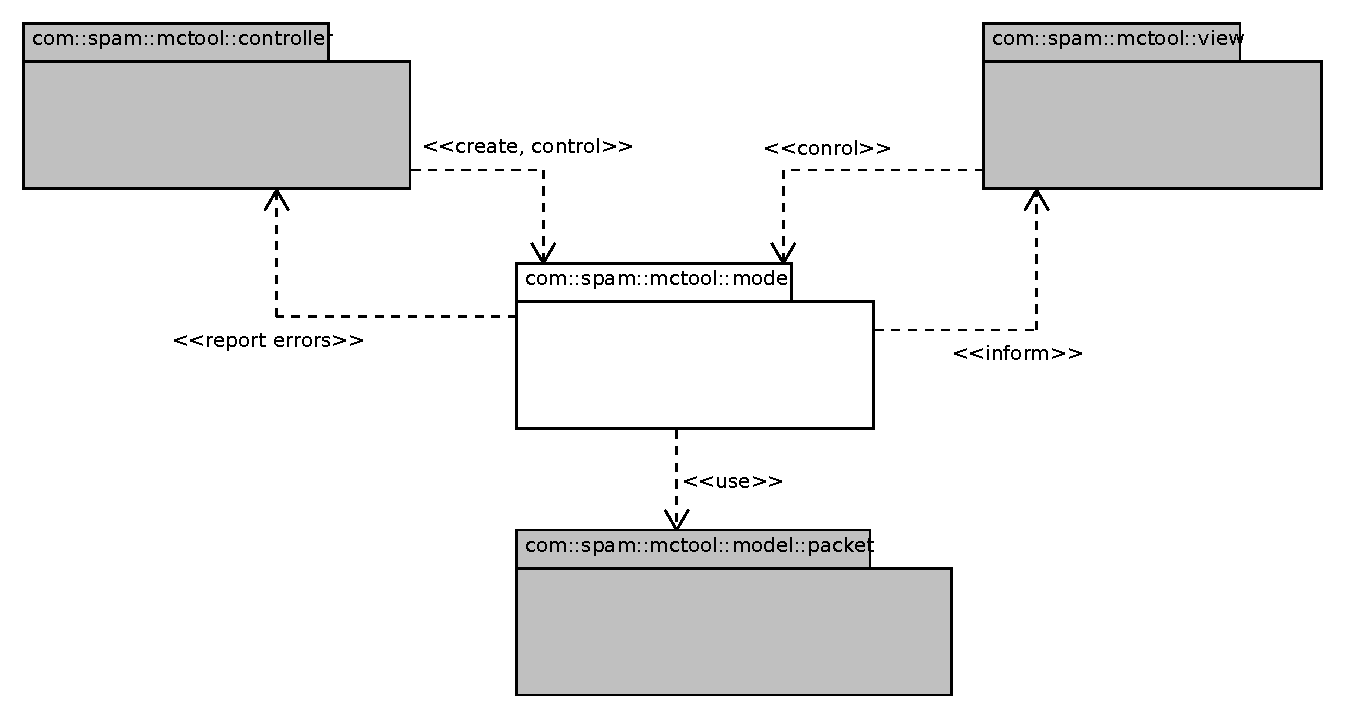
\includegraphics[width=12cm]{images/Einordnung.pdf}
\caption{Einordnung der ESK (weiß) im Gesamtsystem}
\end{figure}

Die ESK bildet den Kern des MTT und kommuniziert deshalb in verschiedenen
Richtungen mit dem Gesamtsystem.

\paragraph{Erzeugung, Steuerung}
Erzeugt und gesteuert wird die ESK direkt von der Steuerkomponente des MTT. Das
Erzeugen erfolgt direkt bei Systemstart, da die ESK zur grundlegenden Funktion
des Systems unabdingbar ist. Die Steuerung umfasst das Anlegen und Löschen von
Datenströmen, sowie Beenden und Ändern der Ausführungsdienste.

\paragraph{Kommunikation}
Aufgabe der ESK ist es Pakete zu versenden und zu empfangen sowie Statistiken
über den erzeugten Datenverkehr aufzubauen. Diese Statistiken werden per
Notify-then-Pull-Verfahren an die Darstellungskomponenten des Systems
weitergegeben. Außerdem informiert die ESK über neue oder gelösche Sender/Empfänger.

\paragraph{Fehlerbehandlung}
Zur Kommunikation von Fehlern zum Benutzer nutzt die ESK die von der
Steuerkomponente bereitgestellte \texttt{ErrorManager}-Schnittstelle verwendet.
Diese bietet die Möglichkeit Fehlermeldungen in verschiedenen Schweregraden an
den Benutzer weitergeben zu können.
Bei Fehlerverhalten versucht die ESK im Allgemeinen die Fehler selbstständig zu
lösen und informiert anschließend den Benutzer über die getroffenen Anpassungen.

\begin{figure}[H]
\center
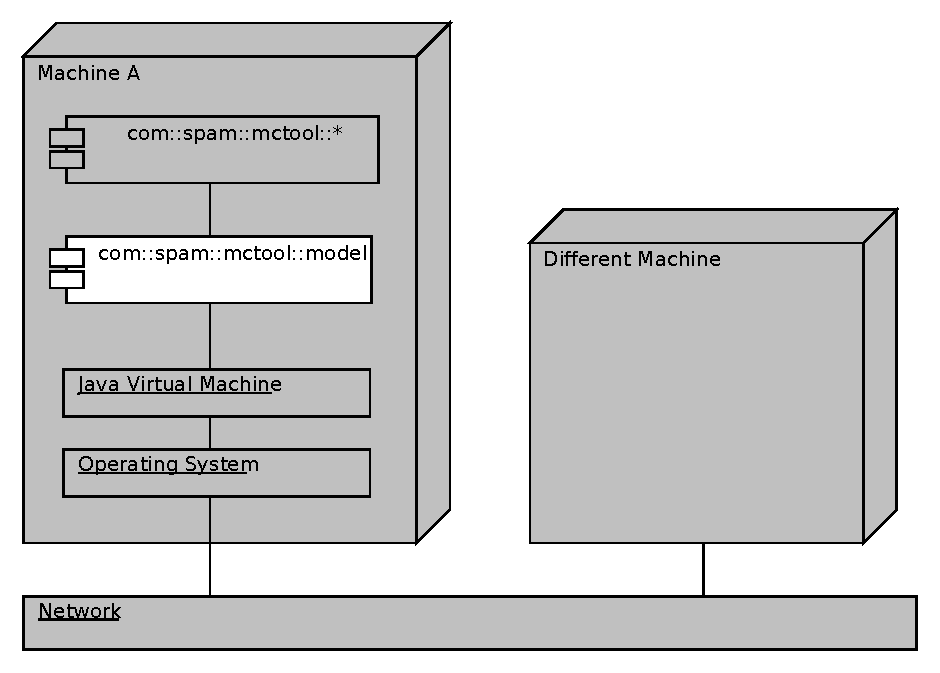
\includegraphics[width=10cm]{images/Verteilungsdiagramm.pdf}
\caption{Einordnung der ESK (weiß), schwarze Linie verdeutlicht den
Informationsfluss}
\end{figure}

\subsection{Problemstellungen}
Problemstellungen die die ESK lösen muss sind folgende:
\begin{enumerate}
  \item Wie kann Multicastdatenverkehr aufgebaut werden?
  \item Wie kann das Senden und Empfangen von Paketen so getakted werden, dass
  bei möglichst vielen Streams die konfigurierten Paket raten erreicht
  werden?
  \item Wie werden neue Datenströme erzeugt?
  \item Wie werden Benutzereingaben validiert?
  \item Wie und wann werden Statistiken über die aufgebauten Datenströme
  errechnet?
  \item Wie und wann werden andere Komponenten über das Vorhandensein neuer
  Statistiken informiert?
\end{enumerate}

Folgende Punkte gehören nicht zum Aufgabenbereich der ESK:
\begin{itemize}
  \item Netzwerkverbindungsmanagement (übernommen von Betriebssystem/Java)
  \item Implementierung von IP, ICMP, UDP Netzwerkprotokollen (übernommen von
  Betriebssystem/Java)
  \item Aufbau der Multicastpakete im Spam- oder Hirschmann-Paketformat
  (übernommen von der Paket-Komponente des Multicast-Test-Tools)
\end{itemize}

\chapter{Design}
%Folgerungen aus der Analyse
%Lösungen für den Problembereich der Analyse
%Systemarchitektur
%Anwendung der Basiskonzepte des Softwareengineerings
%Schnittstellen

\section{Erzeugung der Datenströme}

\begin{figure}[H]
\center
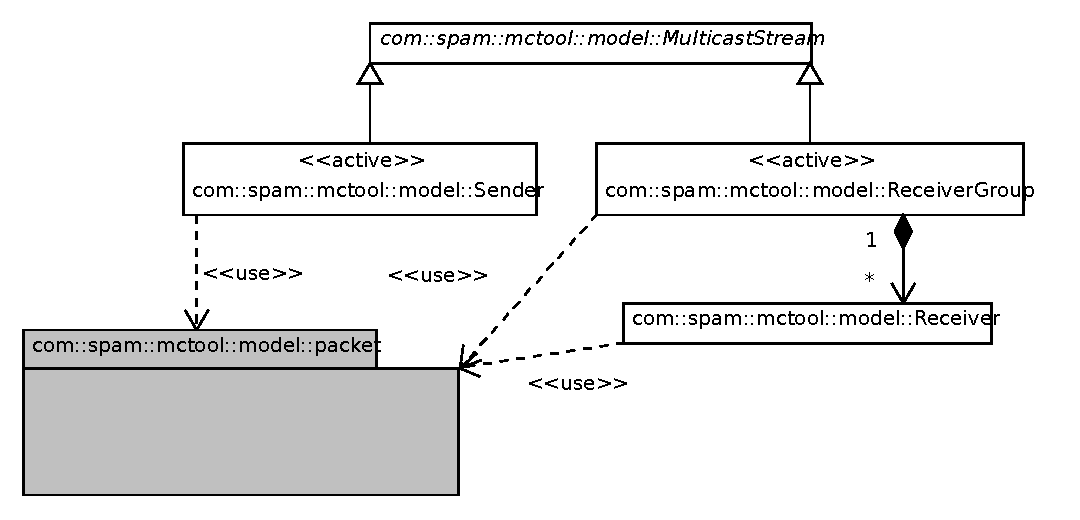
\includegraphics[width=15cm]{images/SR_ov.pdf}
\caption{Übersicht der ESK-Kernklassen (detailiert im Anhang)}
\end{figure}

Wie in oben beschriebener Analyse klar ersichtich ist, besteht die
Grundfunktionalität der ESK im Senden und Empfangen von Datenströmen aus
Multicastpaketen. Dementsprechend ist auch der Kern der ESK in die
entsprechenden Teile für Versand und Empfang aufgeteilt:

\paragraph{\texttt{MutlicastStream}}
Die \texttt{MulticastStream}-Klasse fasst gemeinsame
Multicastdatenstrom-Funktionalitäten in einer gemeinsamen Superklasse zusammen.
Die Hauptfunktion ist das Verwalten einer Netzwerkverbindung
(Netzwerkschnittstelle, Port und Gruppenregistrierung). Auch die Überprüfung der
Konfigurationsparameter findet zum Großteil hier statt.

\paragraph{\texttt{Sender}}
Die \texttt{Sender}-Klasse kommuniziert mit der Paket-Komponente des Systems und
realisiert einen ausgehenden Datenstrom. Dazu ist es wichtig das Versenden der
Pakete sehr genau zu takten, um die eingestellten Paketraten zu erreichen.
Parallel wird zur späteren Auswertung Buch über die tatsächlichen
Paket-Sendezeiten geführt.

\paragraph{\texttt{ReceiverGroup}}
Die \texttt{ReceiverGroup}-Klasse realisiert das Empfangen und teilweise
Auswerten von Multicastpaketen einer bestimmten Multicastgruppe. Da in einer
Gruppe Pakete von vielen Sendern vorhanden sein können, muss der eingehende
Datenstrom weiter aufgeteilt werden. Jede Instanz der Klasse empfängt Pakete
ihrer Gruppe, lässt diese von der Paket-Komponente auswerten und gibt sie dann
an eine Instanz der \texttt{Receiver}-Klasse weiter.

\paragraph{\texttt{Receiver}}
Die \texttt{Receiver}-Klasse stellt das genaue Gegenstück zu einem
\texttt{Sender} in einer bestimmten Multicastgruppe. Jede
\texttt{ReceiverGroup}-Instanz baut für jeden in der Gruppe erkannten Sender
eine \texttt{Receiver}-Instanz auf und übergibt dieser künftig alle empfangenden
Pakete dieses Senders.

Sowohl \texttt{Sender} und \texttt{ReceiverGroup} speichern für die spätere
Auswertung relevante Werte und spezielle Zeitmarken in einer speziellen
Warteschlange.

\section{Auswertung der Messdaten}
Neben dem Senden und Empfangen von Datenströmen muss die ESK die gefordeten
statistischen Werte über alle ein- und ausgehenden Datenströmen erzeugen. Dazu
existiert eine \texttt{SenderAnalyzer} und einer \texttt{ReceiverAnalyzer}
Klasse. Diese sind eng mit ihren Datenstrom-Klassen verbunden und erzeugen in
regelmäßigen Abständen die Statistiken aus den Werten der zuvor aufgebauten
Warteschlange.\\
Um zusätzliche Prozessorauslastung durch unnötige Berechnungen zu vermeiden,
werden Statistiken nur in für menschliche Nutzer relevanten Zeitintervallen
berechnet. Ebenfalls laufen die Berechnungen nur über Stichproben der erfassten
Messdaten.\\
Durch die Zuweisung eines \texttt{AnalyzingBehaviour}s, können die
Zeitintervalle und der Stichprobenumfang beeinflusst werden. Diese passt dabei
ihre Werte automatisch an die Paketraten an, um unter allen Umständen logisch
korrekte Messdaten garantieren zu können.

\section{Kommunikation mit dem System}

\begin{figure}[H]
\center
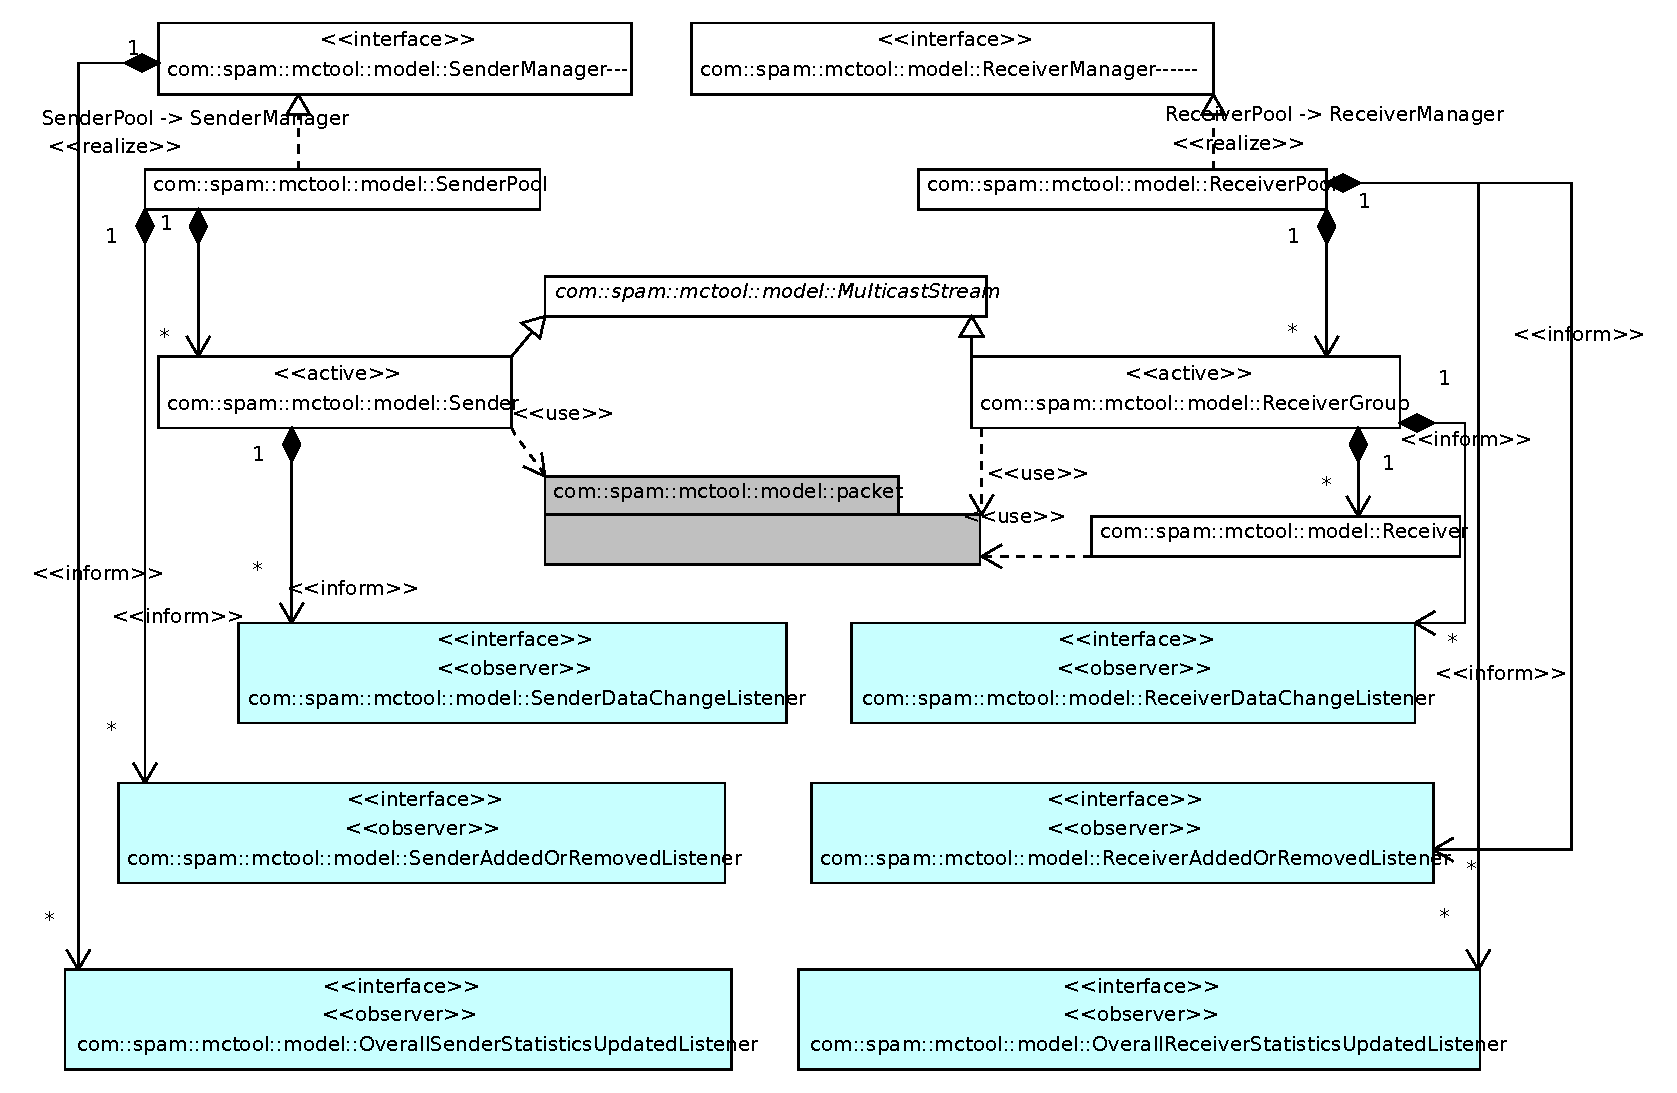
\includegraphics[width=17cm]{images/model_ov.pdf}
\caption{Übersicht des Gesamtmodells (detailiert im Anhang)}
\end{figure}

\subsection{Steuerung}
Sender und Empfänger werden von der Steuer-Komponente des MTT
angelegt oder gelöscht. Die Schnittstellen dafür sind definiert in
\texttt{SenderManager} und \texttt{ReceiverManager}. Bereitgestellt werden sie von den Klassen
\texttt{SenderPool} und \texttt{ReceiverPool}. Diese realisieren folgende
Funktionalitäten:
\begin{itemize}
  \item Paralleles Ausführen der Sender/Empfänger
  \item Anlegen/Löschen von Sendern/Empfängern
  \item Buchführen über alle vorhandenen Sender/Empfänger
  \item Programmweite Statistiken berechnen
\end{itemize}

\subsection{Messdatenverteilung}
Eine wesentliche Aufgabe der ESK neben dem Ausführen der Datenströme ist das
Erstellen und Verteilen von statistischen Informationen. Die ESK informiert über
folgende Ereignisse:
\begin{itemize}
  \item Sender/Empfänger erzeugt/gelöscht
  \item Neue Sender/Empfänger Statistiken
  \item Neue Gesamtstatistiken
\end{itemize}

Die Information wird gemäß
Beobachter-Entwurfsmuster realisiert, folgende sechs Schnittstellen sind dazu
definiert:

\begin{itemize}
  \item
  \texttt{SenderAddedOrRemovedListener}, \texttt{ReceiverAddedOrRemovedListener}
  \item \texttt{SenderDataChangeListener}, \texttt{ReceiverDataChangeListener}
  \item \texttt{OverallSenderStatisticsUpdateListener},
  \texttt{OverallReceiverStatisticsUpdateListener}
\end{itemize}

Klassen die die \texttt{*AddedOrRemovedListener} oder
\texttt{Overall*StatisticsUpdateListener} Schnittstellen implementieren können
sich über Methoden in den \texttt{*Manager}-Schnittstellen für die
entsprechenden Ereignisse registrieren.\\
Klassen, die \texttt{*DataChangeListener} implementieren, müssen sich direkt an
den entsprechenden Datenströmen registrieren.\\
Die registrierenden Klassen werden in regelmäßigen
Abständen durch die ESK informiert.\\
Die betroffenen Datenströme werden dazu in \texttt{Event}-Klassen gekapselt,
diese werden hier aber auf Grund des geringen Funktionsumfangs nicht näher
beleuchtet.

\chapter{Implementierung}
%Vorgehen
%Zwischenergebnisse
%Anwendung der Basiskonzepte
%Codedokumentation
Hier sollen wichtige Punkte der Implementierung der ESK beschrieben werden.
Dieses Dokument kann auf Grund der Größe der Komponente keine vollständige
Beschreibung liefern, für Details sei auf den Programmcode und Javadoc
verwiesen.

\section{Vorgehensweise}
Durch die Voruntersuchungen existierte bereits ein Prototyp der die
grundlegenden Mutlicasting-Funktionen auf Java-Ebene realisierte. Dieser wurde zum Beginn an
die Architektur des MTT angepasst, um eine möglichst frühe
Grundfunktionalität ermöglichen zu können.\\
Im Laufe der Entwicklung wurde der Prototyp dann auf Effizienz optimiert und die
statistischen Auswertungen implementiert.

\section{Erzeugen von Sendern und Empfängern}
Die Datenströme werden direkt von der Steuerkomponente des MTT erzeugt oder
gelöscht. Dazu bietet die \texttt{*Manager}-Schnittstellen
\texttt{create()}-Methoden die Hashmaps mit Werten entgegennehmen. Die Werte
werden validiert (zum Großteil von \texttt{MulticastStream}, Sender oder
Empfänger spezifische Werte von den entsprechenden Klassen). Bei Erfolg wird der
erzeugte Sender (Empfänger) zurückgeliefert. Dieser bietet selbst die Methoden
zum (De-)Aktivieren an.

\section{Erzeugung der Datenströme}

\subsection{Executor-Framework}
Um die Anforderungen an Effizienz und Skalierbarkeit möglichst gut zu erfüllen,
ist das Senden und Empfangen von Multicastpaketen mit dem
Executor-Entwurfsmuster realisiert.

\begin{figure}[H]
\center
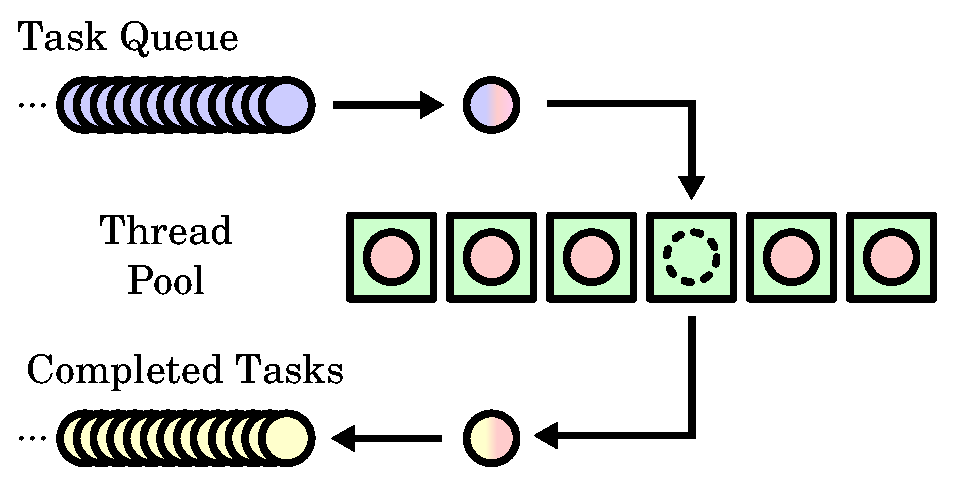
\includegraphics[width=10cm]{images/threadpool.pdf}
\caption{Prinzip des Executer-Entwurfmusters, Quelle: Wikipedia}
\end{figure}

Beim Executor-Entwurfsmuster wird eine Menge von Arbeits-Prozessen
(Worker-Threads) aufgebaut. Parallel dazu werden Aufgaben gesammelt und
nacheinander von den Worker-Threads abgearbeitet. Dadurch wird der Mehraufwand
für das ständige Erzeugen von Prozessen eingespart und eine relativ konstante
Prozessor-Auslastung garantiert.

Java bietet für diesen Zweck das sogenannte Java Concurrency Framework
(JCF) an. Durch Verwendungen dieser nativen Java-Komponente wird versucht, die
von der Virtualisierung ausgehenden Geschwindigkeitseinbusen von Java
einzudämmen.

\subsection{Realisierung}
Sowohl die \texttt{Sender} als auch die \texttt{ReceiverGroup} implementieren
die \texttt{Runnable}-Schnittstelle von Java. Damit qualifizieren sie sich als
Arbeitspakete für das Executor-Framework. Beide Klassen beinhalten ebenfalls jeweils eine
eingebettete Klasse \texttt{*Analyzer} die ebenfalls eine Realisation von
\texttt{Runnable} ist und in regelmäßigen Abständen ausgeführt wird um die
Statistiken des Datenstroms zu berechnen. Der
Aufzählungstyp \texttt{AnalyzingBehaviour} kann in drei Variatonen beeinflussen
in welchen Zeitabständen die Statistiken neu berechnet werden. Dadurch wird die
Prozessor-Auslastung durch unnötige Berechnungen reduziert.

\begin{figure}[H]
\center
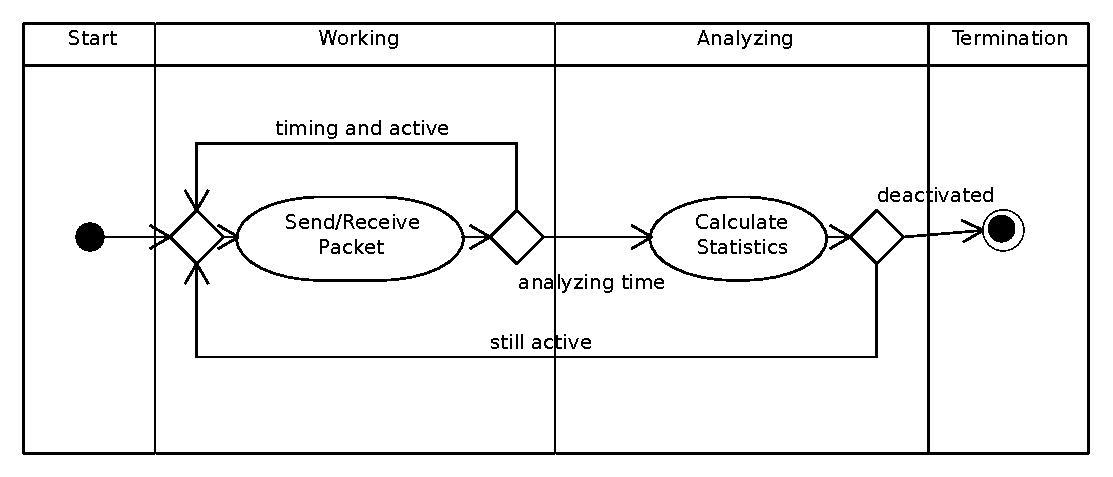
\includegraphics[width=10cm]{images/datastream.pdf}
\caption{Verhalten eines Datenstroms}
\end{figure}

Die eigentlichen Threadpools befinden sich in \texttt{SenderPool} und
\texttt{ReceiverPool}. Ihre Größe kann dynamisch verändert werden um das
Laufzeitverhalten an Systeme mit unterschiedlichen Prozessorkernanzahlen
anpassen zu können.

\subsection{Beenden der Datenströme}
Das Beenden von Datenströmen gestaltet sich nicht so trivial wie es auf den
ersten Blick erscheinen mag. Dadurch, dass pro Klasse zwei aktive Threads
exisitieren, müssen diese auch koordiniert beendet werden. Der verwendete
Thread-Pool erzeugt dafür für jede geplante Aufgaben ein sogenanntes
\texttt{Future}-Objekt, mit dem die Aufgabe abgebrochen werden kann. Auf
Empfänger-Seite kann es zu Socket-Exceptions kommen, wenn der Netzwerksocket
geschlossen wird bevor der empfangende Thread beendet wurde. Diese Fehler sind
nach Ermessen des Entwicklers unerheblich.

\section{Verteilung von Daten}
Um andere Komponenten des Systems über Ereignisse wie neu errechnete Messdaten
oder neue/entfernte Datenströme zu informieren, wird ausschließlich das
Beobachter-Entwurfsmuster verwendet. Komponenten die über bestimme Ereignisse
informiert werden wollten, implementieren die entsprechenden Schnittstellen und
registieren sich an den \texttt{*Pools} bzw an \texttt{Sender} oder
\texttt{Receiver} direkt.\\
Sobald neue Daten vorliegen, werden diese in \texttt{Events} verpackt und an die
Schnittstellen-Methoden der registrierten Observer übergeben. Diese können die
Daten dann nach eigenem Ermessen weiterverarbeiten.


\chapter{Komponententest}
%Wie wird die Komponente getestet?
%Dokumentation von Vorgehen und Ergebnissen. Bei Bedarf entsprechend erweitern
Durch die Parallelität und Abhängigkeiten vom Netzwerksystem des
Host-Systems sind automatisierte Komponenten-Tests nur sehr schwer zu
realisieren. Da jedoch bei fast jedem Systemtest eine exakte Funktionalität der
ESK mitabgeprüft wird, sei hautpsächlich auf diese verwiesen.\\[1cm]

Die betreffenden Testsuiten lauten:
\begin{itemize}
  \item TS10, Parametervalidierung und Funktionalität von Sendern
  \item TS20, Parametervalidierung und Funktionalität von Empfängern
  \item TS50, Validierung der Mutlicasting-Fähigkeiten
  \item TS60, Korrektheit der erzeugten Statistiken
\end{itemize}
Für deren Beschreibung sei zwecks Vermeidung von Redundanz auf den STP
verwiesen.\\
Die Testergebnisse sind im STR nachzulesen - zusammenfassend soll hier gesagt
werden dass alle Tests erfolgreich abgeschlossen werden konnten.

\section{Komponententestplan}
Trotz der schweren automatisierten Testbarkeit, sind die wichtigtsten
Funktionalitäten mit JUnit Tests abgedeckt worden.

\begin{table}[h]
\caption{Komponententestplan}
\label{tab:ktp}
\begin{center}
\begin{tabular}{|p{2cm}|p{5cm}|p{5cm}|}
\hline
\textbf{Testcase} & \textbf{Beschreibung} & \textbf{Klasse}\\
\hline
MTC01 & Funktionalität der Buffer-Queue sicherstellen & LinkedSplitQueueTest\\
\hline
MTC02 & Wichtigste Werteüberprüfungen für Benutzereingaben sicherstellen &
MulticastStreamTest \\
\hline
MTC03 & Funktionalität des ReceiverPools sicherstellen & ReceiverPoolTest\\
\hline
MTC04 & Funktionalität des SenderPools sicherstellen & SenderPoolTest \\
\hline
MTC05 & Statistische Auswertung des Empfängers sicherstellen & ReceiverTest \\
\hline
\end{tabular}
\end{center}
\end{table}

\section{Komponententestreport}

\begin{table}[h]
\caption{Komponententestreport}
\label{tab:ktr}
\begin{center}
\begin{tabular}{|p{2cm}|p{2cm}|p{6cm}|p{1.5cm}|p{1.5cm}|}
\hline
\textbf{Test Nr.} & \textbf{Pass/Fail} & \textbf{Test Ergebnis (wenn Fail)} & \textbf{Datum} & \textbf{Tester}\\
\hline
MTC01 & Pass & - & 10.05.2011 & JJ\\
\hline
MTC02 & Pass & - & 10.05.2011 & JJ\\
\hline
MTC03 & Pass & - & 10.05.2011 & JJ\\
\hline
MTC04 & Pass & - & 10.05.2011 & JJ\\
\hline
MTC05 & Pass & - & 10.05.2011 & JJ\\
\hline
\end{tabular}
\end{center}
\end{table}

\chapter{Zusammenfassung}

\section{Beurteilung der Komponente}
%Hat die Komponente Schwächen und Stärken,
%Besonderheiten?
%Übertragbarkeit der Komponente und Lösungen
%Was ist verbesserungswürdig?
\paragraph{Stärken}
Die klare Stärke der ESK besteht in der Parallelität, die durch Verwendung des
Thread-Pool-Entwurfsmusters sowohl für Datenstromversand bzw -empfang als auch
für die Berechnung der Statistiken erreicht wird.\\
Durch Anpassen der Größe dieses Pools, kann die Leistungsfähigkeit des Tools
auf jede Hardware, vom normalen Heimcomputer bis zum Mehrkern-Server, skaliert
werden.\\
Da die Kommunikation mit dem restlichen System ausschließlich über
Beobachter-Entwurfsmuster realisiert wird, können beliebig viele
unterschiedliche Komponenten über die erzeugten Ereignisse informiert werden.

\paragraph{Schwächen}
Eine Schwäche der ESK ist, dass durch die starke Parallelisierung der Komponente
und Abhängigkeit vom Netzwerk das Hostsystems, autmatisierte Tests nahezu nicht
möglich sind.\\
Durch die relativ komplexe Implementierung ist mit einer erschwerten Wartbarkeit
zu rechnen.

\paragraph{Weiterentwicklung}
Durch Auslagerung der Paketkomponente, ist es in Zukunft möglich, beliebige
andere Paket-Formate im MTT zu integrieren. Damit wäre sogar ein
Nutzdatenübertragung per Mutlicast denkbar.\\
Davon abgesehen befolgt das Design der ESK alle anerkannten Designprinzipien und
bietet dadurch eine allgemeine gute Wartbarkeit.\\
Konkrete Erweiterungen sind derzeit nicht geplant.


\chapter{Referenzen und Standards}
SRS - System Requirements Specification\\
SAS - System Architecture Specification\\
STP - System Test Plan\\
STR - System Test Report\\
MCTOOL - Programmcode und Javadoc\\